\ECchapter{02}{Hydrogen}{Can hydrogen decarbonise heavy transport?}{ECBlue}

\ECObjectives{
\begin{itemize}[leftmargin=*,itemsep=1pt,topsep=1pt]
\item Distinguish grey, blue and green hydrogen.
\item Explain the operating principles of electrolysers and fuel cells.
\item Compare hydrogen and battery-electric energy chains.
\end{itemize}}

\begin{multicols}{2}

\begin{engineeringnews}
Low-emission hydrogen projects are being developed for fertiliser production, steel,
shipping and heavy road transport. Their success depends not only on electrolyser
capacity, but also on electricity supply, storage, transport and final demand.
\end{engineeringnews}

\begin{ecarticle}
Hydrogen is an \textbf{energy carrier}, not a primary source of energy. It must be
manufactured from another resource before it can be stored and used. Most hydrogen is
still produced from natural gas by steam methane reforming. If the resulting carbon
dioxide is released, the product is called grey hydrogen. Capturing part of the CO$_2$
leads to so-called blue hydrogen. Green hydrogen is produced by electrolysis powered by
low-carbon renewable electricity.

In a proton-exchange-membrane (PEM) electrolyser, water enters the anode side. An
electric current separates the water molecules into oxygen, protons and electrons. The
membrane allows protons to cross while forcing electrons through an external circuit.
Hydrogen is formed at the cathode.

A PEM fuel cell performs the reverse overall reaction. Hydrogen is supplied to the
anode and oxygen from air reaches the cathode. The electrochemical reaction produces
electricity, water and heat without combustion. Several cells are assembled in a stack
to obtain the required voltage and power.

Hydrogen has a high specific energy by mass and enables rapid refuelling. However, its
low volumetric density requires compression, liquefaction or conversion into another
carrier. Each conversion consumes energy. Consequently, a battery-electric vehicle is
usually more efficient from electricity source to wheels, while hydrogen can remain
attractive when long range, high payload and short refuelling stops are essential.
\end{ecarticle}

\begin{tcolorbox}[colback=white,colframe=ECBlue,title=\sffamily\bfseries PEM electrolyser]
\centering
\begin{tikzpicture}[font=\scriptsize,>=Latex,node distance=5mm]
\node[draw,rounded corners,minimum width=23mm,minimum height=17mm,fill=blue!5] (an) {\shortstack{Anode\\$2H_2O\rightarrow O_2+4H^++4e^-$}};
\node[draw,minimum width=7mm,minimum height=17mm,fill=yellow!20,right=of an] (mem) {PEM};
\node[draw,rounded corners,minimum width=23mm,minimum height=17mm,fill=green!7,right=of mem] (cat) {\shortstack{Cathode\\$4H^++4e^-\rightarrow2H_2$}};
\draw[->,thick] (an) -- node[above] {$H^+$} (mem);
\draw[->,thick] (mem) -- node[above] {$H^+$} (cat);
\draw[->,thick] ([yshift=-5mm]an.south) -- ++(0,-4mm) -| node[pos=.25,below] {$e^-$ through DC supply} ([yshift=-5mm]cat.south);
\draw[<-] (an.west) -- ++(-7mm,0) node[left] {$H_2O$};
\draw[->] ([yshift=4mm]an.west) -- ++(-7mm,0) node[left] {$O_2$};
\draw[->] (cat.east) -- ++(7mm,0) node[right] {$H_2$};
\end{tikzpicture}
\end{tcolorbox}

\columnbreak

\begin{engineeringfocus}
\textbf{The complete hydrogen value chain}
\begin{enumerate}[leftmargin=*,itemsep=1pt]
\item Generate low-carbon electricity.
\item Produce hydrogen by electrolysis.
\item Purify and compress the gas.
\item Store and distribute it safely.
\item Convert it into useful energy in a fuel cell or industrial process.
\end{enumerate}
Engineers optimise efficiency, safety, materials, cost and infrastructure at every
stage. Hydrogen leaks must also be controlled because the molecule is very small and
has a wide flammability range in air.
\end{engineeringfocus}

\begin{tcolorbox}[colback=white,colframe=ECBlue,title=\sffamily\bfseries PEM fuel cell]
\centering
\begin{tikzpicture}[font=\scriptsize,>=Latex,node distance=5mm]
\node[draw,rounded corners,minimum width=23mm,minimum height=17mm,fill=green!7] (an) {\shortstack{Anode\\$2H_2\rightarrow4H^++4e^-$}};
\node[draw,minimum width=7mm,minimum height=17mm,fill=yellow!20,right=of an] (mem) {PEM};
\node[draw,rounded corners,minimum width=23mm,minimum height=17mm,fill=blue!5,right=of mem] (cat) {\shortstack{Cathode\\$O_2+4H^++4e^-\rightarrow2H_2O$}};
\draw[->,thick] (an) -- node[above] {$H^+$} (mem);
\draw[->,thick] (mem) -- node[above] {$H^+$} (cat);
\draw[->,thick] ([yshift=-5mm]an.south) -- ++(0,-4mm) -| node[pos=.25,below] {electrical load} ([yshift=-5mm]cat.south);
\draw[<-] (an.west) -- ++(-7mm,0) node[left] {$H_2$};
\draw[<-] (cat.east) -- ++(7mm,0) node[right] {air};
\draw[->] ([yshift=4mm]cat.east) -- ++(7mm,0) node[right] {$H_2O$};
\end{tikzpicture}
\end{tcolorbox}

\begin{tcolorbox}[colback=white,colframe=ECBlue,title=\sffamily\bfseries Electricity-to-wheel efficiency]
\centering
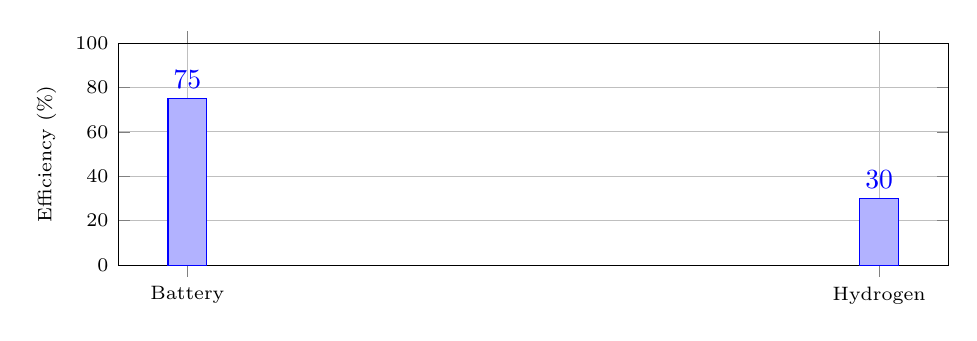
\begin{tikzpicture}
\begin{axis}[
width=\linewidth,height=44mm,
ybar,bar width=14pt,
ymin=0,ymax=100,
ylabel={Efficiency (\%)},
symbolic x coords={Battery,Hydrogen},xtick=data,
nodes near coords,
grid=major,
tick label style={font=\scriptsize},label style={font=\scriptsize}]
\addplot coordinates {(Battery,75) (Hydrogen,30)};
\end{axis}
\end{tikzpicture}

{\scriptsize Illustrative whole-chain values; actual performance depends on equipment and operating conditions.}
\end{tcolorbox}

\begin{tcolorbox}[colback=yellow!10,colframe=ECOrange,title=\sffamily\bfseries Did You Know?]
Hydrogen contains about 120 MJ of energy per kilogram on a lower-heating-value basis,
but storing one kilogram requires a much larger tank than storing an equivalent amount
of liquid fuel.
\end{tcolorbox}

\begin{tcolorbox}[colback=blue!5,colframe=ECBlue,title=\sffamily\bfseries Key Figures]
\begin{tabularx}{\linewidth}{@{}Xr@{}}
Hydrogen LHV & $\approx120$ MJ/kg\\
Electrolyser efficiency & 60--75\%\\
Fuel-cell electrical efficiency & 40--60\%\\
Typical vehicle storage pressure & 350 or 700 bar
\end{tabularx}
\end{tcolorbox}

\begin{vocabulary}
\begin{tabularx}{\linewidth}{@{}lX@{}}
electrolyser & électrolyseur\\
fuel cell & pile à combustible\\
stack & empilement de cellules\\
compressed gas & gaz comprimé\\
refuelling & ravitaillement\\
leak detection & détection de fuite
\end{tabularx}
\end{vocabulary}

\begin{questions}
\item Why is hydrogen described as an energy carrier?
\item Compare grey, blue and green hydrogen.
\item Explain the role of the PEM in an electrolyser.
\item What products leave a fuel cell?
\item Why is the battery chain usually more efficient?
\item In which transport applications can hydrogen remain attractive?
\end{questions}

\begin{challenge}
A logistics company operates 120 long-haul trucks. Compare battery-electric and
hydrogen fuel-cell solutions using efficiency, range, payload, refuelling time,
infrastructure and lifecycle emissions. Present a justified engineering recommendation.
\end{challenge}

\begin{applicationexercise}
An electrolyser consumes 52~kWh of electricity to produce 1~kg of hydrogen. A fuel-cell
system later converts the hydrogen into 18~kWh of useful electrical energy. Calculate the
power-to-power efficiency of this chain. Compare it with an 88\% battery storage system and
explain why hydrogen may still be selected for some applications.
\end{applicationexercise}

\begin{speaking}
Debate: ``Hydrogen will replace batteries for heavy transport.'' Each team must use at
least three technical arguments and respond to one opposing argument.
\end{speaking}

\end{multicols}

\subsection*{Sources and further reading}
\small
\ECsource{IEA — Global Hydrogen Review}{https://www.iea.org/reports/global-hydrogen-review-2024};
\ECsource{U.S. Department of Energy — Hydrogen and Fuel Cell Technologies Office}{https://www.energy.gov/eere/fuelcells/hydrogen-and-fuel-cell-technologies-office};
\ECsource{European Commission — Hydrogen}{https://energy.ec.europa.eu/topics/eus-energy-system/hydrogen_en}.

\medskip
\qrcode[height=16mm]{https://www.iea.org/reports/global-hydrogen-review-2024}
\hspace{5mm}
\qrcode[height=16mm]{https://www.energy.gov/eere/fuelcells/hydrogen-and-fuel-technologies-office}
